\section{Chain A -- Periodic ID Publisher}

Generates a random integer $\mathit{id}\in[0,30000]$ together with the
current UNIX timestamp once per second, publishes the JSON payload to
\texttt{challenge3/id\_generator}, and appends the same fields to
\texttt{id\_log.csv}.

\begin{figure}[h]
    \centering
    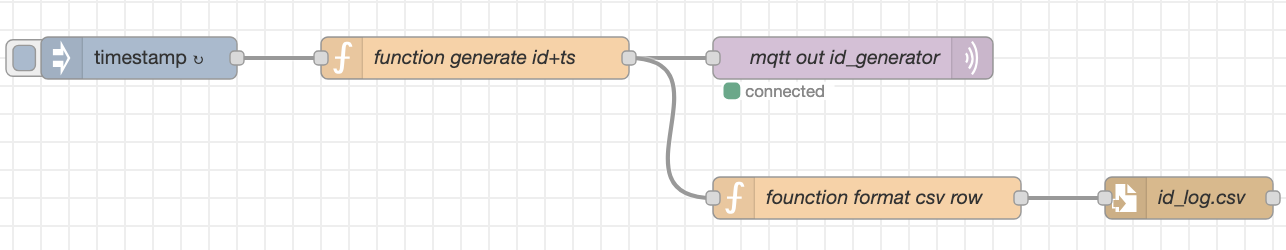
\includegraphics[width=0.85\linewidth]{images/flow_chain_a.png}
    \caption{Chain A -- ID generator and CSV logger.}
\end{figure}

\begin{description}
    \item[timestamp] fires a tick every second.
    \item[function \emph{generate id+ts}] builds the payload
        \verb|{id, timestamp}| as a JavaScript object that Node-RED
        serialises automatically. A flow-context counter stops the
        publisher after exactly 200 ticks, keeping \texttt{id\_log.csv}
        bounded.
        \begin{lstlisting}[caption={Generate ID + timestamp}, label={lst:gen}]
        // Stop publishing after 200 messages
        let pubCount = flow.get('pubCount') || 0;
        if (pubCount >= 200) return null;
        flow.set('pubCount', pubCount + 1);
        
        const id = Math.floor(Math.random() * 30001);
        const timestamp = Math.floor(Date.now() / 1000);
        msg.payload = { id: id, timestamp: timestamp };
        return msg;
        \end{lstlisting}
    \item[mqtt out id\_generator] publishes to topic \texttt{challenge3/id\_generator}
        on \texttt{localhost:1884}.
    \item[function \emph{format csv row}] keeps an incremental row counter
        in the flow context, prepends the header on the first row, and
        emits a newline-terminated CSV line.
        \begin{lstlisting}[caption={Format CSV row}]
        let rowNum = flow.get('idLogRowNum') || 0;
        rowNum++;
        flow.set('idLogRowNum', rowNum);
        
        let line = '';
        if (rowNum === 1) line = 'No.,ID,TIMESTAMP\n';
        line += `${rowNum},${msg.payload.id},${msg.payload.timestamp}\n`;
        
        msg.payload = line;
        return msg;
        \end{lstlisting}
    \item[File (append)] appends each line to \texttt{id\_log.csv}.
\end{description}
